% Evaluation criterion:
%- Language and use of figures
%- Clarity of the problem statement
%- Overall document structure
%- Depth of understanding for the field of computer architecture
%- Depth of understanding of the investigated problem

\section{Result}
\label{sec:result}

The speedup from when running the selected applications with the
different prefetchers is tabulated in \autoref{fig:initResults}.
% These speedups are calculated from stats from m5... Don't need this
% here, have already written this in methodology/intro - right?

\begin{figure}[ht]
  \centering
  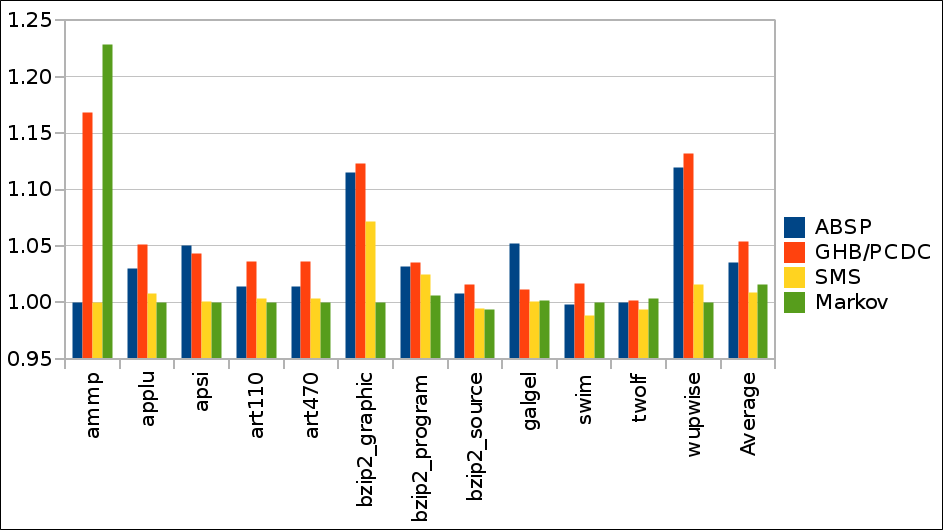
\includegraphics[scale=0.25]{figures/init_results.png}
  \caption{\label{fig:initResults} Speedup on the Y-axis plotted
    against program on the X-axis.}
\end{figure}

Detailed data of the results from the optimal parameter search as
described in \autoref{sec:methodology} is not included, being just an
intermediate step towards performing a just comparison of the
different prefetchers.

%What other results? Should we include parameter search results? What
%about results from experimenting with altering the prefetchers---does
%that belong here or in the discussion section?XS
%
%\subsection{Sequential Prefetcher Result}
%\label{sec:sequentialPrefetcherResult}
%
%\subsection{GHB Prefetcher Result}
%\label{sec:ghbPrefetcherResult}
%
%\subsection{Markov Prefetcher Result}
%\label{sec:markovPrefetcherResult}
%
%\subsection{Spatial Memory Streaming Prefetcher Result}
%\label{sec:smsPrefetcherResult}

